% Options for packages loaded elsewhere
\PassOptionsToPackage{unicode}{hyperref}
\PassOptionsToPackage{hyphens}{url}
\PassOptionsToPackage{dvipsnames,svgnames,x11names}{xcolor}
%
\documentclass[
  10pt,
  letterpaper,
  DIV=11,
  numbers=noendperiod]{scrartcl}

\usepackage{amsmath,amssymb}
\usepackage{setspace}
\usepackage{iftex}
\ifPDFTeX
  \usepackage[T1]{fontenc}
  \usepackage[utf8]{inputenc}
  \usepackage{textcomp} % provide euro and other symbols
\else % if luatex or xetex
  \usepackage{unicode-math}
  \defaultfontfeatures{Scale=MatchLowercase}
  \defaultfontfeatures[\rmfamily]{Ligatures=TeX,Scale=1}
\fi
\usepackage{lmodern}
\ifPDFTeX\else  
    % xetex/luatex font selection
  \setmonofont[Scale=0.75]{Source Code Pro}
\fi
% Use upquote if available, for straight quotes in verbatim environments
\IfFileExists{upquote.sty}{\usepackage{upquote}}{}
\IfFileExists{microtype.sty}{% use microtype if available
  \usepackage[]{microtype}
  \UseMicrotypeSet[protrusion]{basicmath} % disable protrusion for tt fonts
}{}
\makeatletter
\@ifundefined{KOMAClassName}{% if non-KOMA class
  \IfFileExists{parskip.sty}{%
    \usepackage{parskip}
  }{% else
    \setlength{\parindent}{0pt}
    \setlength{\parskip}{6pt plus 2pt minus 1pt}}
}{% if KOMA class
  \KOMAoptions{parskip=half}}
\makeatother
\usepackage{xcolor}
\setlength{\emergencystretch}{3em} % prevent overfull lines
\setcounter{secnumdepth}{-\maxdimen} % remove section numbering
% Make \paragraph and \subparagraph free-standing
\ifx\paragraph\undefined\else
  \let\oldparagraph\paragraph
  \renewcommand{\paragraph}[1]{\oldparagraph{#1}\mbox{}}
\fi
\ifx\subparagraph\undefined\else
  \let\oldsubparagraph\subparagraph
  \renewcommand{\subparagraph}[1]{\oldsubparagraph{#1}\mbox{}}
\fi

\usepackage{color}
\usepackage{fancyvrb}
\newcommand{\VerbBar}{|}
\newcommand{\VERB}{\Verb[commandchars=\\\{\}]}
\DefineVerbatimEnvironment{Highlighting}{Verbatim}{commandchars=\\\{\}}
% Add ',fontsize=\small' for more characters per line
\usepackage{framed}
\definecolor{shadecolor}{RGB}{241,243,245}
\newenvironment{Shaded}{\begin{snugshade}}{\end{snugshade}}
\newcommand{\AlertTok}[1]{\textcolor[rgb]{0.68,0.00,0.00}{#1}}
\newcommand{\AnnotationTok}[1]{\textcolor[rgb]{0.37,0.37,0.37}{#1}}
\newcommand{\AttributeTok}[1]{\textcolor[rgb]{0.40,0.45,0.13}{#1}}
\newcommand{\BaseNTok}[1]{\textcolor[rgb]{0.68,0.00,0.00}{#1}}
\newcommand{\BuiltInTok}[1]{\textcolor[rgb]{0.00,0.23,0.31}{#1}}
\newcommand{\CharTok}[1]{\textcolor[rgb]{0.13,0.47,0.30}{#1}}
\newcommand{\CommentTok}[1]{\textcolor[rgb]{0.37,0.37,0.37}{#1}}
\newcommand{\CommentVarTok}[1]{\textcolor[rgb]{0.37,0.37,0.37}{\textit{#1}}}
\newcommand{\ConstantTok}[1]{\textcolor[rgb]{0.56,0.35,0.01}{#1}}
\newcommand{\ControlFlowTok}[1]{\textcolor[rgb]{0.00,0.23,0.31}{#1}}
\newcommand{\DataTypeTok}[1]{\textcolor[rgb]{0.68,0.00,0.00}{#1}}
\newcommand{\DecValTok}[1]{\textcolor[rgb]{0.68,0.00,0.00}{#1}}
\newcommand{\DocumentationTok}[1]{\textcolor[rgb]{0.37,0.37,0.37}{\textit{#1}}}
\newcommand{\ErrorTok}[1]{\textcolor[rgb]{0.68,0.00,0.00}{#1}}
\newcommand{\ExtensionTok}[1]{\textcolor[rgb]{0.00,0.23,0.31}{#1}}
\newcommand{\FloatTok}[1]{\textcolor[rgb]{0.68,0.00,0.00}{#1}}
\newcommand{\FunctionTok}[1]{\textcolor[rgb]{0.28,0.35,0.67}{#1}}
\newcommand{\ImportTok}[1]{\textcolor[rgb]{0.00,0.46,0.62}{#1}}
\newcommand{\InformationTok}[1]{\textcolor[rgb]{0.37,0.37,0.37}{#1}}
\newcommand{\KeywordTok}[1]{\textcolor[rgb]{0.00,0.23,0.31}{#1}}
\newcommand{\NormalTok}[1]{\textcolor[rgb]{0.00,0.23,0.31}{#1}}
\newcommand{\OperatorTok}[1]{\textcolor[rgb]{0.37,0.37,0.37}{#1}}
\newcommand{\OtherTok}[1]{\textcolor[rgb]{0.00,0.23,0.31}{#1}}
\newcommand{\PreprocessorTok}[1]{\textcolor[rgb]{0.68,0.00,0.00}{#1}}
\newcommand{\RegionMarkerTok}[1]{\textcolor[rgb]{0.00,0.23,0.31}{#1}}
\newcommand{\SpecialCharTok}[1]{\textcolor[rgb]{0.37,0.37,0.37}{#1}}
\newcommand{\SpecialStringTok}[1]{\textcolor[rgb]{0.13,0.47,0.30}{#1}}
\newcommand{\StringTok}[1]{\textcolor[rgb]{0.13,0.47,0.30}{#1}}
\newcommand{\VariableTok}[1]{\textcolor[rgb]{0.07,0.07,0.07}{#1}}
\newcommand{\VerbatimStringTok}[1]{\textcolor[rgb]{0.13,0.47,0.30}{#1}}
\newcommand{\WarningTok}[1]{\textcolor[rgb]{0.37,0.37,0.37}{\textit{#1}}}

\providecommand{\tightlist}{%
  \setlength{\itemsep}{0pt}\setlength{\parskip}{0pt}}\usepackage{longtable,booktabs,array}
\usepackage{calc} % for calculating minipage widths
% Correct order of tables after \paragraph or \subparagraph
\usepackage{etoolbox}
\makeatletter
\patchcmd\longtable{\par}{\if@noskipsec\mbox{}\fi\par}{}{}
\makeatother
% Allow footnotes in longtable head/foot
\IfFileExists{footnotehyper.sty}{\usepackage{footnotehyper}}{\usepackage{footnote}}
\makesavenoteenv{longtable}
\usepackage{graphicx}
\makeatletter
\def\maxwidth{\ifdim\Gin@nat@width>\linewidth\linewidth\else\Gin@nat@width\fi}
\def\maxheight{\ifdim\Gin@nat@height>\textheight\textheight\else\Gin@nat@height\fi}
\makeatother
% Scale images if necessary, so that they will not overflow the page
% margins by default, and it is still possible to overwrite the defaults
% using explicit options in \includegraphics[width, height, ...]{}
\setkeys{Gin}{width=\maxwidth,height=\maxheight,keepaspectratio}
% Set default figure placement to htbp
\makeatletter
\def\fps@figure{htbp}
\makeatother

% packages
\usepackage{geometry}
\usepackage{xcolor}
\usepackage{eso-pic}
\usepackage{fancyhdr}
\usepackage{sectsty}
\usepackage{fontspec}
\usepackage{titlesec}
% \usepackage{lmodern}
% \usepackage{cmbright}
\usepackage{fvextra}

\DefineVerbatimEnvironment{Highlighting}{Verbatim}{breaklines,commandchars=\\\{\}}
\DefineVerbatimEnvironment{OutputCode}{Verbatim}{breaklines,commandchars=\\\{\}}

% use sans serif font
% \renewcommand{\familydefault}{\sfdefault}

%% colours
\definecolor{primary}{HTML}{FCEDE2}
\definecolor{dark}{HTML}{330033}

%% fontsize
\addtokomafont{subsubsection}{\fontsize{10pt}{12.833pt}\selectfont}



%% Add the border
\AddToShipoutPicture{% 
    \AtPageLowerLeft{% 
        \put(\LenToUnit{\dimexpr\paperwidth-2cm},0){% 
            \color{primary}\rule{2cm}{\LenToUnit\paperheight}%
          }%
     }%
     % logo
    \AtPageLowerLeft{% start the bar at the bottom right of the page
        \put(\LenToUnit{\dimexpr\paperwidth-1.75cm},\paperheight-2.5cm){% move it to the top right
            \color{primary}
\includegraphics[width=1.5cm]{_extensions/soles-assignment/assets/images/usydlogo.png}
          }%
     }%
}

%% Style the page number
\fancypagestyle{usyd}{
  \fancyhf{}
  \renewcommand\headrulewidth{0pt}
  \fancyfoot[R]{\thepage}
  \fancyfootoffset{3.5cm}
}
\setlength{\footskip}{20pt}

%% style the chapter/section fonts
\chapterfont{\color{dark}\fontsize{20}{16.8}\selectfont}
\sectionfont{\color{dark}\fontsize{20}{16.8}\selectfont}
\subsectionfont{\color{dark}\fontsize{14}{16.8}\selectfont}
\titleformat{\subsection}
  {\sffamily\Large\bfseries}{\thesection}{1em}{}[{\titlerule[0.8pt]}]
  
% left align title
\makeatletter
\renewcommand{\maketitle}{\bgroup\setlength{\parindent}{0pt}
\begin{flushleft}
  {\sffamily\huge\textbf{\MakeUppercase{\@title}}} \vspace{0.3cm} \newline
  {\Large {\@subtitle}} \newline
  \@author
\end{flushleft}\egroup
}
\makeatother
\KOMAoption{captions}{tableheading}
\makeatletter
\@ifpackageloaded{tcolorbox}{}{\usepackage[skins,breakable]{tcolorbox}}
\@ifpackageloaded{fontawesome5}{}{\usepackage{fontawesome5}}
\definecolor{quarto-callout-color}{HTML}{909090}
\definecolor{quarto-callout-note-color}{HTML}{0758E5}
\definecolor{quarto-callout-important-color}{HTML}{CC1914}
\definecolor{quarto-callout-warning-color}{HTML}{EB9113}
\definecolor{quarto-callout-tip-color}{HTML}{00A047}
\definecolor{quarto-callout-caution-color}{HTML}{FC5300}
\definecolor{quarto-callout-color-frame}{HTML}{acacac}
\definecolor{quarto-callout-note-color-frame}{HTML}{4582ec}
\definecolor{quarto-callout-important-color-frame}{HTML}{d9534f}
\definecolor{quarto-callout-warning-color-frame}{HTML}{f0ad4e}
\definecolor{quarto-callout-tip-color-frame}{HTML}{02b875}
\definecolor{quarto-callout-caution-color-frame}{HTML}{fd7e14}
\makeatother
\makeatletter
\makeatother
\makeatletter
\makeatother
\makeatletter
\@ifpackageloaded{caption}{}{\usepackage{caption}}
\AtBeginDocument{%
\ifdefined\contentsname
  \renewcommand*\contentsname{Table of contents}
\else
  \newcommand\contentsname{Table of contents}
\fi
\ifdefined\listfigurename
  \renewcommand*\listfigurename{List of Figures}
\else
  \newcommand\listfigurename{List of Figures}
\fi
\ifdefined\listtablename
  \renewcommand*\listtablename{List of Tables}
\else
  \newcommand\listtablename{List of Tables}
\fi
\ifdefined\figurename
  \renewcommand*\figurename{Figure}
\else
  \newcommand\figurename{Figure}
\fi
\ifdefined\tablename
  \renewcommand*\tablename{Table}
\else
  \newcommand\tablename{Table}
\fi
}
\@ifpackageloaded{float}{}{\usepackage{float}}
\floatstyle{ruled}
\@ifundefined{c@chapter}{\newfloat{codelisting}{h}{lop}}{\newfloat{codelisting}{h}{lop}[chapter]}
\floatname{codelisting}{Listing}
\newcommand*\listoflistings{\listof{codelisting}{List of Listings}}
\makeatother
\makeatletter
\@ifpackageloaded{caption}{}{\usepackage{caption}}
\@ifpackageloaded{subcaption}{}{\usepackage{subcaption}}
\makeatother
\makeatletter
\@ifpackageloaded{tcolorbox}{}{\usepackage[skins,breakable]{tcolorbox}}
\makeatother
\makeatletter
\@ifundefined{shadecolor}{\definecolor{shadecolor}{HTML}{e64626}}
\makeatother
\makeatletter
\@ifundefined{codebgcolor}{\definecolor{codebgcolor}{HTML}{F1F1F1}}
\makeatother
\makeatletter
\makeatother
\ifLuaTeX
  \usepackage{selnolig}  % disable illegal ligatures
\fi
\IfFileExists{bookmark.sty}{\usepackage{bookmark}}{\usepackage{hyperref}}
\IfFileExists{xurl.sty}{\usepackage{xurl}}{} % add URL line breaks if available
\urlstyle{same} % disable monospaced font for URLs
\hypersetup{
  pdftitle={ENVX2001 Lab 07 - Regression model development},
  colorlinks=true,
  linkcolor={blue},
  filecolor={Maroon},
  citecolor={Blue},
  urlcolor={Blue},
  pdfcreator={LaTeX via pandoc}}

\title{ENVX2001 Lab 07 - Regression model development}
\author{}
\date{Semester 1, 2024}

\begin{document}
\maketitle
\pagestyle{usyd}

\ifdefined\Shaded\renewenvironment{Shaded}{\begin{tcolorbox}[colback={codebgcolor}, borderline west={3pt}{0pt}{shadecolor}, enhanced, breakable, frame hidden, sharp corners, boxrule=0pt]}{\end{tcolorbox}}\fi

\renewcommand*\contentsname{Table of contents}
{
\hypersetup{linkcolor=}
\setcounter{tocdepth}{3}
\tableofcontents
}
\setstretch{1.2}
\begin{tcolorbox}[enhanced jigsaw, rightrule=.15mm, coltitle=black, leftrule=.75mm, titlerule=0mm, breakable, toprule=.15mm, bottomtitle=1mm, colback=white, toptitle=1mm, opacitybacktitle=0.6, bottomrule=.15mm, arc=.35mm, left=2mm, title=\textcolor{quarto-callout-tip-color}{\faLightbulb}\hspace{0.5em}{Tip}, colbacktitle=quarto-callout-tip-color!10!white, opacityback=0, colframe=quarto-callout-tip-color-frame]

Please work on this exercise by creating your own R Markdown file.

\end{tcolorbox}

\hypertarget{exercise-1-bird-abundance}{%
\subsection{Exercise 1: Bird
abundance}\label{exercise-1-bird-abundance}}

This is the \emph{same} dataset used in the lecture.

Fragmentation of forest habitat has an impact of wildlife abundance.
This study looked at the relationship between bird abundance (bird
ha\textsuperscript{-1}) and the characteristics of forest patches at 56
locations in SE Victoria.

The predictor variables are:

\begin{itemize}
\tightlist
\item
  \texttt{ALT} Altitude (m)
\item
  \texttt{YR.ISOL} Year when the patch was isolated (years)
\item
  \texttt{GRAZE} Grazing (coded 1-5 which is light to heavy)
\item
  \texttt{AREA} Patch area (ha)
\item
  \texttt{DIST} Distance to nearest patch (km)
\item
  \texttt{LDIST} Distance to largest patch (km)
\end{itemize}

Import the data from the ``Loyn'' tab in the MS Excel file.

\begin{Shaded}
\begin{Highlighting}[]
\FunctionTok{library}\NormalTok{(readxl)}
\NormalTok{loyn }\OtherTok{\textless{}{-}} \FunctionTok{read\_xlsx}\NormalTok{(}\StringTok{"mlr.xlsx"}\NormalTok{, }\StringTok{"Loyn"}\NormalTok{)}
\end{Highlighting}
\end{Shaded}

Often, the first step in model development is to examine the data. This
is a good way to get a feel for the data and to identify any issues that
may need to be addressed. In this case, we will examine the data using
histograms and a correlation matrix.

\hypertarget{histograms}{%
\subsubsection{Histograms}\label{histograms}}

There are a breadth of ways to create histograms in R. In each tab below
you will find some different ways to create the same plot outputs.

\subsection{\texorpdfstring{\texttt{hist()}}{hist()}}

This is a straightforward way to create multiple histograms with
\texttt{hist()}. The \texttt{par()} function is used to arrange the
plots on the page. The \texttt{mfrow} argument specifies the number of
rows and columns of plots.

\begin{Shaded}
\begin{Highlighting}[]
\CommentTok{\#par(mfrow=c(3,3))}
\FunctionTok{hist}\NormalTok{(loyn}\SpecialCharTok{$}\NormalTok{ABUND)}
\end{Highlighting}
\end{Shaded}

\begin{figure}[H]

{\centering 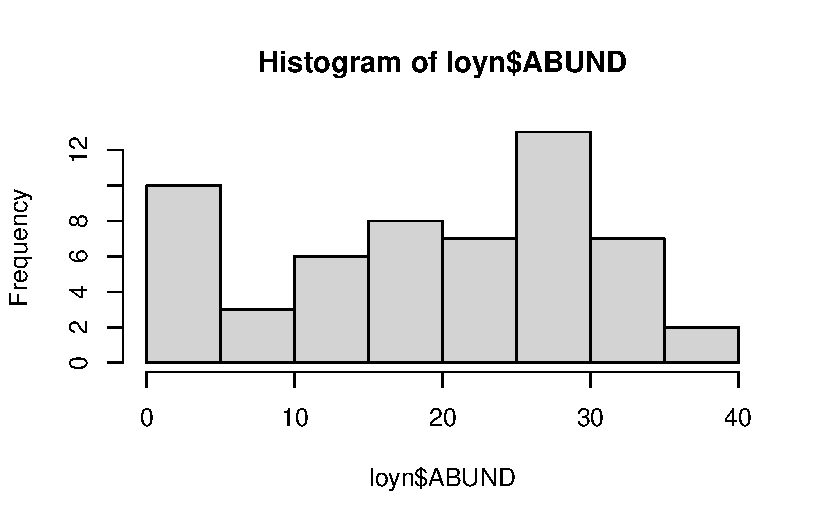
\includegraphics{ENVX2001-2024-Lab07_files/figure-pdf/unnamed-chunk-2-1.pdf}

}

\end{figure}

\begin{Shaded}
\begin{Highlighting}[]
\FunctionTok{hist}\NormalTok{(loyn}\SpecialCharTok{$}\NormalTok{ALT)}
\end{Highlighting}
\end{Shaded}

\begin{figure}[H]

{\centering 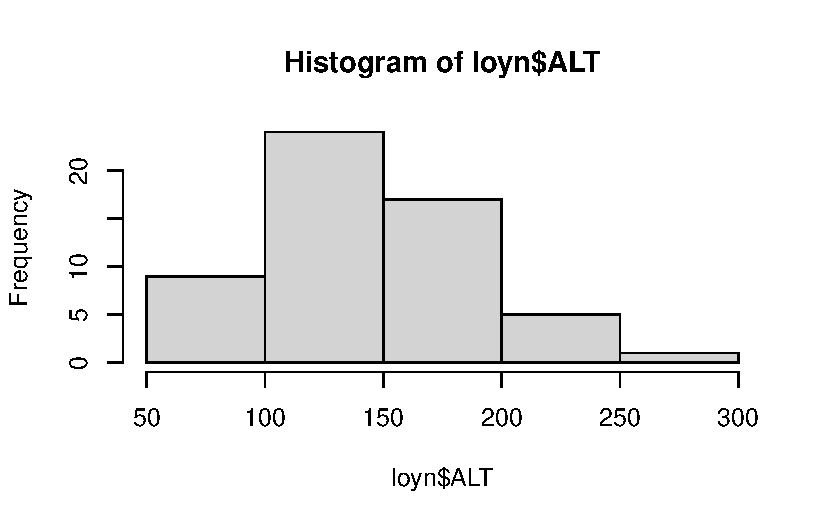
\includegraphics{ENVX2001-2024-Lab07_files/figure-pdf/unnamed-chunk-2-2.pdf}

}

\end{figure}

\begin{Shaded}
\begin{Highlighting}[]
\FunctionTok{hist}\NormalTok{(loyn}\SpecialCharTok{$}\NormalTok{YR.ISOL)}
\end{Highlighting}
\end{Shaded}

\begin{figure}[H]

{\centering 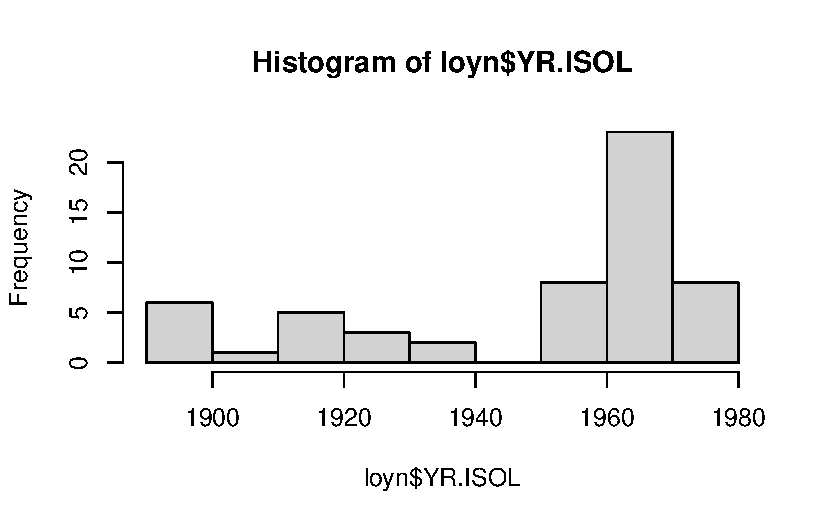
\includegraphics{ENVX2001-2024-Lab07_files/figure-pdf/unnamed-chunk-2-3.pdf}

}

\end{figure}

\begin{Shaded}
\begin{Highlighting}[]
\FunctionTok{hist}\NormalTok{(loyn}\SpecialCharTok{$}\NormalTok{GRAZE)}
\end{Highlighting}
\end{Shaded}

\begin{figure}[H]

{\centering 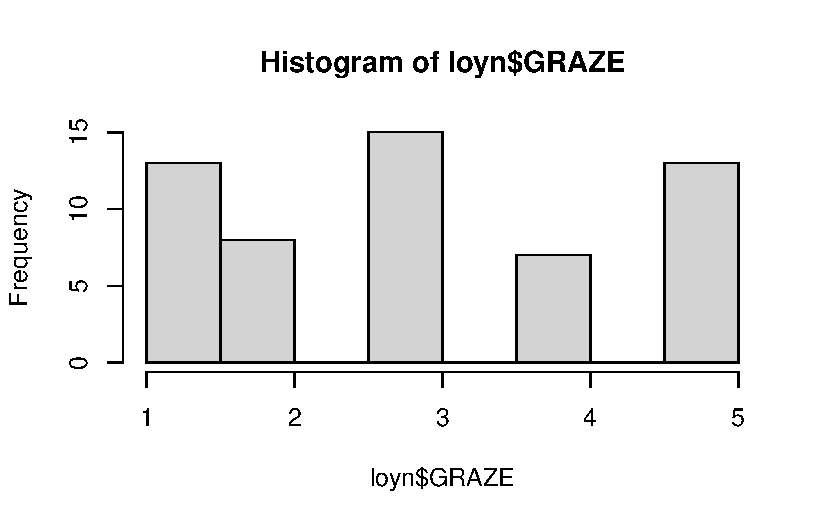
\includegraphics{ENVX2001-2024-Lab07_files/figure-pdf/unnamed-chunk-2-4.pdf}

}

\end{figure}

\begin{Shaded}
\begin{Highlighting}[]
\FunctionTok{hist}\NormalTok{(loyn}\SpecialCharTok{$}\NormalTok{AREA)}
\end{Highlighting}
\end{Shaded}

\begin{figure}[H]

{\centering 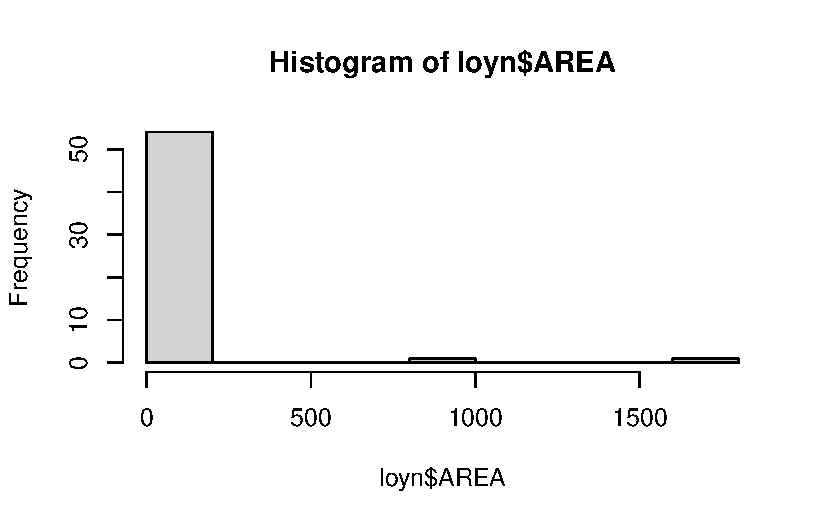
\includegraphics{ENVX2001-2024-Lab07_files/figure-pdf/unnamed-chunk-2-5.pdf}

}

\end{figure}

\begin{Shaded}
\begin{Highlighting}[]
\FunctionTok{hist}\NormalTok{(loyn}\SpecialCharTok{$}\NormalTok{DIST)}
\end{Highlighting}
\end{Shaded}

\begin{figure}[H]

{\centering 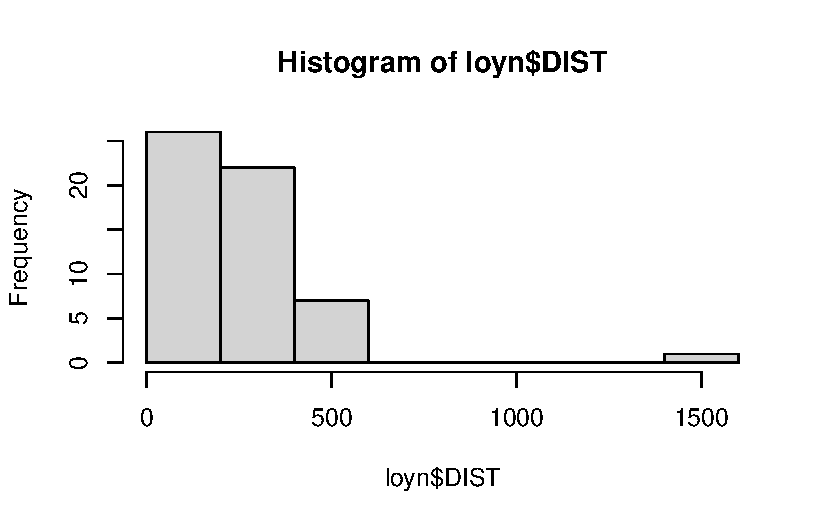
\includegraphics{ENVX2001-2024-Lab07_files/figure-pdf/unnamed-chunk-2-6.pdf}

}

\end{figure}

\begin{Shaded}
\begin{Highlighting}[]
\FunctionTok{hist}\NormalTok{(loyn}\SpecialCharTok{$}\NormalTok{LDIST)}
\end{Highlighting}
\end{Shaded}

\begin{figure}[H]

{\centering 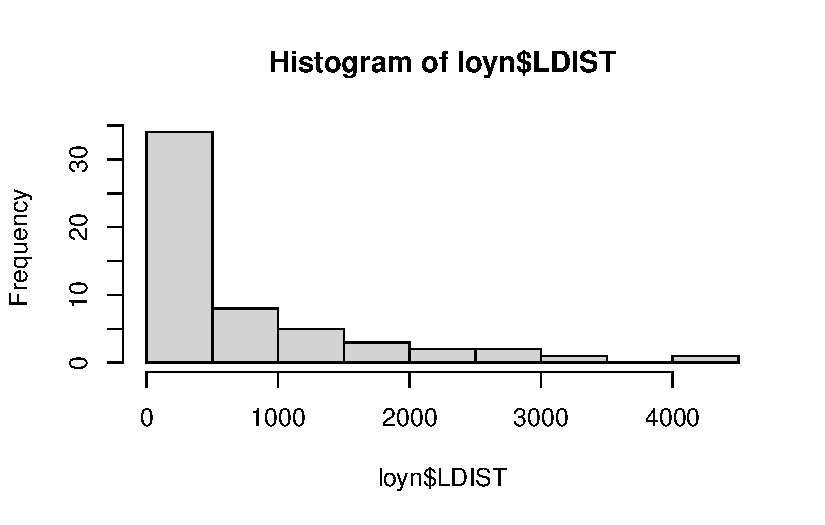
\includegraphics{ENVX2001-2024-Lab07_files/figure-pdf/unnamed-chunk-2-7.pdf}

}

\end{figure}

\begin{Shaded}
\begin{Highlighting}[]
\CommentTok{\#par(mfrow=c(1,1))}
\end{Highlighting}
\end{Shaded}

\subsection{\texorpdfstring{\texttt{hist.data.frame()} from
\texttt{Hmisc}}{hist.data.frame() from Hmisc}}

The \texttt{Hmisc} package provides a function
\texttt{hist.data.frame()} that can be used to create multiple
histograms, which can be called by simply using \texttt{hist()}. You may
need to tweak the \texttt{nclass} argument to get the desired number of
bins, as the default may not look appropriate.

\begin{Shaded}
\begin{Highlighting}[]
\CommentTok{\# install.packages("Hmisc")}
\FunctionTok{library}\NormalTok{(Hmisc)}
\FunctionTok{hist}\NormalTok{(loyn, }\AttributeTok{nclass =} \DecValTok{50}\NormalTok{)}
\end{Highlighting}
\end{Shaded}

\subsection{\texorpdfstring{\texttt{ggplot()}}{ggplot()}}

A more modern approach is to use \texttt{ggplot()} with
\texttt{facet\_wrap()} to arrange multiple plots on a single page. To do
this, the \texttt{pivot\_longer()} function from the \texttt{tidyr}
package is used to reshape the data into a tidy format.

\begin{Shaded}
\begin{Highlighting}[]
\CommentTok{\# tidy the data}
\NormalTok{loyn\_tidy }\OtherTok{\textless{}{-}} \FunctionTok{pivot\_longer}\NormalTok{(loyn, }\AttributeTok{cols =} \FunctionTok{everything}\NormalTok{())}

\CommentTok{\# plot}
\FunctionTok{ggplot}\NormalTok{(loyn\_tidy, }\FunctionTok{aes}\NormalTok{(}\AttributeTok{x =}\NormalTok{ value)) }\SpecialCharTok{+} 
  \FunctionTok{geom\_histogram}\NormalTok{() }\SpecialCharTok{+} 
  \FunctionTok{facet\_wrap}\NormalTok{(}\SpecialCharTok{\textasciitilde{}}\NormalTok{name, }\AttributeTok{scales =} \StringTok{"free"}\NormalTok{) }\SpecialCharTok{+}
  \FunctionTok{theme\_bw}\NormalTok{()}
\end{Highlighting}
\end{Shaded}

\begin{figure}[H]

{\centering 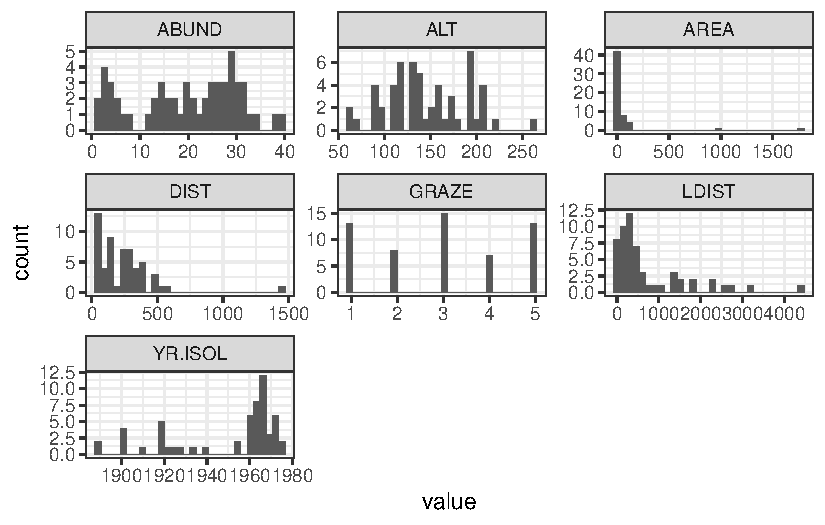
\includegraphics{ENVX2001-2024-Lab07_files/figure-pdf/unnamed-chunk-4-1.pdf}

}

\end{figure}

\subsection{\texorpdfstring{\texttt{ggplot()} with
\texttt{dplyr}}{ggplot() with dplyr}}

Here we use the pipe operator \texttt{\%\textgreater{}\%} from
\texttt{dplyr} to chain together a series of commands. The pipe operator
takes the output of the command on the left and passes it to the command
on the right (or below) the pipe. This means that we can create a series
of commands that are executed in order.

\begin{Shaded}
\begin{Highlighting}[]
\NormalTok{loyn }\SpecialCharTok{\%\textgreater{}\%} 
  \FunctionTok{pivot\_longer}\NormalTok{(}\AttributeTok{cols =} \FunctionTok{everything}\NormalTok{()) }\SpecialCharTok{\%\textgreater{}\%} 
  \FunctionTok{ggplot}\NormalTok{(}\FunctionTok{aes}\NormalTok{(}\AttributeTok{x =}\NormalTok{ value)) }\SpecialCharTok{+} 
  \FunctionTok{geom\_histogram}\NormalTok{() }\SpecialCharTok{+} 
  \FunctionTok{facet\_wrap}\NormalTok{(}\SpecialCharTok{\textasciitilde{}}\NormalTok{name, }\AttributeTok{scales =} \StringTok{"free"}\NormalTok{) }\SpecialCharTok{+}
  \FunctionTok{theme\_bw}\NormalTok{()}
\end{Highlighting}
\end{Shaded}

\begin{figure}[H]

{\centering 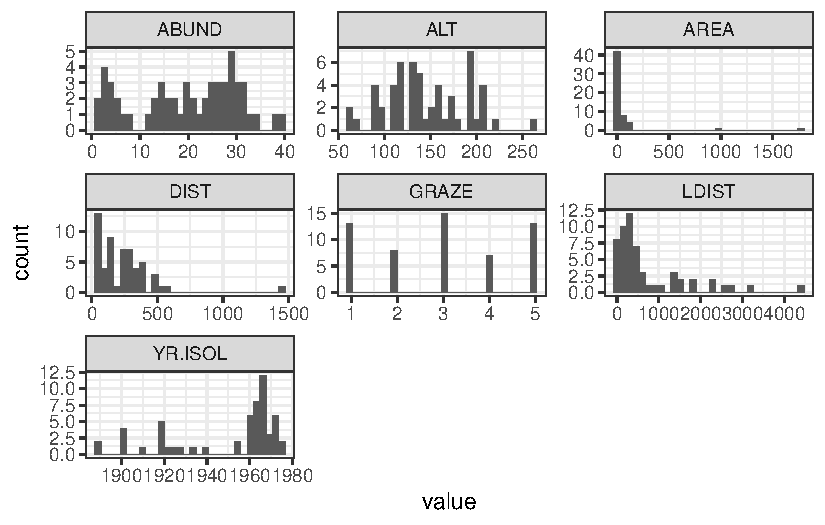
\includegraphics{ENVX2001-2024-Lab07_files/figure-pdf/unnamed-chunk-5-1.pdf}

}

\end{figure}

\begin{tcolorbox}[enhanced jigsaw, rightrule=.15mm, coltitle=black, leftrule=.75mm, titlerule=0mm, breakable, toprule=.15mm, bottomtitle=1mm, colback=white, toptitle=1mm, opacitybacktitle=0.6, bottomrule=.15mm, arc=.35mm, left=2mm, title=\textcolor{quarto-callout-warning-color}{\faExclamationTriangle}\hspace{0.5em}{Question 1}, colbacktitle=quarto-callout-warning-color!10!white, opacityback=0, colframe=quarto-callout-warning-color-frame]

Comment on the histograms in terms of leverage. \emph{Hint: what is the
relationship between leverage and skewness?}

\end{tcolorbox}

\hypertarget{answer}{%
\subsection{Answer}\label{answer}}

The histograms of \texttt{AREA}, \texttt{DIST} and \texttt{LDIST} are
very skewed. The high values would have high leverage, this means that
these would cause the residuals to be skewed. These would be candidates
for transformation.

\hypertarget{correlation-matrix}{%
\subsubsection{Correlation matrix}\label{correlation-matrix}}

Calculate the correlation matrix using \texttt{cor(Loyn)}.

\begin{Shaded}
\begin{Highlighting}[]
\FunctionTok{cor}\NormalTok{(loyn)}
\end{Highlighting}
\end{Shaded}

\begin{verbatim}
              ABUND         AREA      YR.ISOL       DIST       LDIST
ABUND    1.00000000  0.255970206  0.503357741  0.2361125  0.08715258
AREA     0.25597021  1.000000000 -0.001494192  0.1083429  0.03458035
YR.ISOL  0.50335774 -0.001494192  1.000000000  0.1132175 -0.08331686
DIST     0.23611248  0.108342870  0.113217524  1.0000000  0.31717234
LDIST    0.08715258  0.034580346 -0.083316857  0.3171723  1.00000000
GRAZE   -0.68251138 -0.310402417 -0.635567104 -0.2558418 -0.02800944
ALT      0.38583617  0.387753885  0.232715406 -0.1101125 -0.30602220
              GRAZE        ALT
ABUND   -0.68251138  0.3858362
AREA    -0.31040242  0.3877539
YR.ISOL -0.63556710  0.2327154
DIST    -0.25584182 -0.1101125
LDIST   -0.02800944 -0.3060222
GRAZE    1.00000000 -0.4071671
ALT     -0.40716705  1.0000000
\end{verbatim}

\begin{tcolorbox}[enhanced jigsaw, rightrule=.15mm, coltitle=black, leftrule=.75mm, titlerule=0mm, breakable, toprule=.15mm, bottomtitle=1mm, colback=white, toptitle=1mm, opacitybacktitle=0.6, bottomrule=.15mm, arc=.35mm, left=2mm, title=\textcolor{quarto-callout-warning-color}{\faExclamationTriangle}\hspace{0.5em}{Question 2}, colbacktitle=quarto-callout-warning-color!10!white, opacityback=0, colframe=quarto-callout-warning-color-frame]

Which independent variables are useful for predicting the dependent
variable abundance? Is there evidence for multi-collinearity?

\end{tcolorbox}

\hypertarget{answer-1}{%
\subsection{Answer}\label{answer-1}}

Some of the predictors are useful, but AREA has a low r.

The correlation between \texttt{GRAZE} and \texttt{YR.ISOL} is quite
high (r = -0.63556710), suggesting multi-collinearity which may
influence the model. If the relationship between these two variables was
stronger, we would remove one of the variables to prevent this
collinearity from affecting the model.

\emph{Note: For more information on collinearity and how it may impact
the model, see Quinn \& Keough p 127.}

\hypertarget{plotting-correlation}{%
\subsubsection{Plotting correlation}\label{plotting-correlation}}

Examine correlations visually using \texttt{pairs()} or
\texttt{corrplot()} from the \texttt{corrplot} package.

\subsection{Scatterplot matrix}

\begin{Shaded}
\begin{Highlighting}[]
\FunctionTok{pairs}\NormalTok{(loyn)}
\end{Highlighting}
\end{Shaded}

\begin{figure}[H]

{\centering 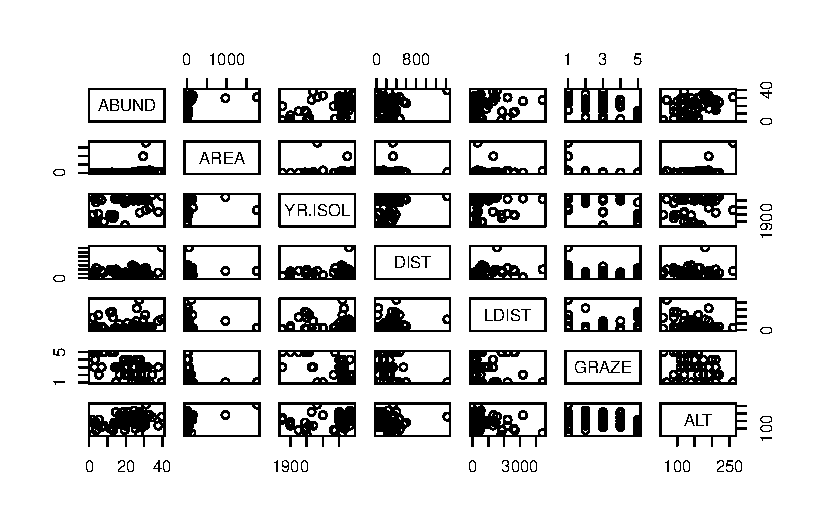
\includegraphics{ENVX2001-2024-Lab07_files/figure-pdf/unnamed-chunk-7-1.pdf}

}

\end{figure}

\subsection{Correlation matrix}

\begin{Shaded}
\begin{Highlighting}[]
\FunctionTok{library}\NormalTok{(corrplot)}
\FunctionTok{corrplot}\NormalTok{(}\FunctionTok{cor}\NormalTok{(loyn))}
\end{Highlighting}
\end{Shaded}

\begin{figure}[H]

{\centering 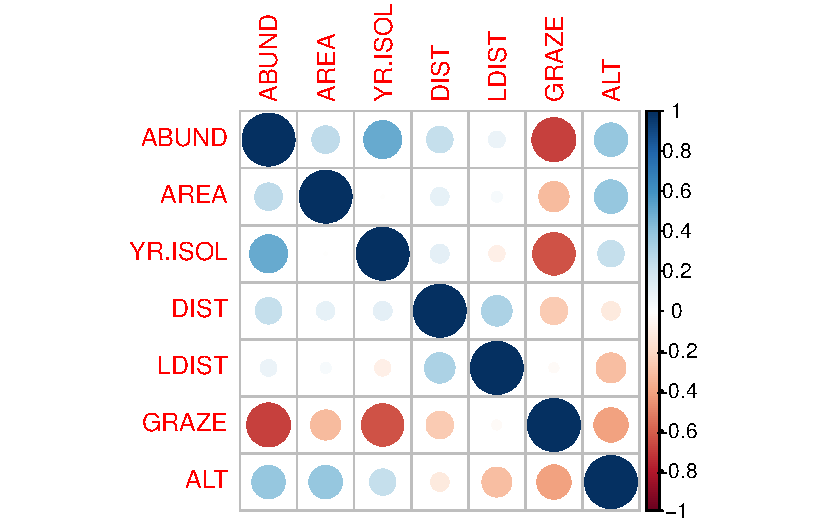
\includegraphics{ENVX2001-2024-Lab07_files/figure-pdf/unnamed-chunk-8-1.pdf}

}

\end{figure}

\begin{tcolorbox}[enhanced jigsaw, rightrule=.15mm, coltitle=black, leftrule=.75mm, titlerule=0mm, breakable, toprule=.15mm, bottomtitle=1mm, colback=white, toptitle=1mm, opacitybacktitle=0.6, bottomrule=.15mm, arc=.35mm, left=2mm, title=\textcolor{quarto-callout-warning-color}{\faExclamationTriangle}\hspace{0.5em}{Question 3}, colbacktitle=quarto-callout-warning-color!10!white, opacityback=0, colframe=quarto-callout-warning-color-frame]

Are there any trends visible from the plots?

\end{tcolorbox}

\hypertarget{answer-2}{%
\subsection{Answer}\label{answer-2}}

Not really; the pairs plot reflects the strength of the linear
relationship between each of the variables. There may be some stronger
relationships occurring, but it is evident a few of the variables are
skewed so it is harder to distinguish within the plots.

\begin{tcolorbox}[enhanced jigsaw, rightrule=.15mm, coltitle=black, leftrule=.75mm, titlerule=0mm, breakable, toprule=.15mm, bottomtitle=1mm, colback=white, toptitle=1mm, opacitybacktitle=0.6, bottomrule=.15mm, arc=.35mm, left=2mm, title=\textcolor{quarto-callout-tip-color}{\faLightbulb}\hspace{0.5em}{Tip}, colbacktitle=quarto-callout-tip-color!10!white, opacityback=0, colframe=quarto-callout-tip-color-frame]

We can also bring in variance inflation factors (VIF) to help us
identify multi-collinearity, but that is done only after we have
selected a model.

\end{tcolorbox}

\hypertarget{transformations}{%
\subsubsection{Transformations}\label{transformations}}

The AREA predictor has a small number of observations with very large
values. Apply a log\textsubscript{10} transformation and label the new
variable \texttt{Loyn\$L10AREA}.

\begin{Shaded}
\begin{Highlighting}[]
\NormalTok{loyn}\SpecialCharTok{$}\NormalTok{L10AREA }\OtherTok{\textless{}{-}} \FunctionTok{log10}\NormalTok{(loyn}\SpecialCharTok{$}\NormalTok{AREA)}
\end{Highlighting}
\end{Shaded}

\begin{tcolorbox}[enhanced jigsaw, rightrule=.15mm, coltitle=black, leftrule=.75mm, titlerule=0mm, breakable, toprule=.15mm, bottomtitle=1mm, colback=white, toptitle=1mm, opacitybacktitle=0.6, bottomrule=.15mm, arc=.35mm, left=2mm, title=\textcolor{quarto-callout-warning-color}{\faExclamationTriangle}\hspace{0.5em}{Question 4}, colbacktitle=quarto-callout-warning-color!10!white, opacityback=0, colframe=quarto-callout-warning-color-frame]

Why are we transforming AREA?

\end{tcolorbox}

\hypertarget{answer-3}{%
\subsection{Answer}\label{answer-3}}

You do this to stabilise the variance of the regression to manage the
leverage of the outliers in the variable. This reduces the skew. L10AREA
is more likely to be a significant predictor.

\begin{tcolorbox}[enhanced jigsaw, rightrule=.15mm, coltitle=black, leftrule=.75mm, titlerule=0mm, breakable, toprule=.15mm, bottomtitle=1mm, colback=white, toptitle=1mm, opacitybacktitle=0.6, bottomrule=.15mm, arc=.35mm, left=2mm, title=\textcolor{quarto-callout-warning-color}{\faExclamationTriangle}\hspace{0.5em}{Question 5}, colbacktitle=quarto-callout-warning-color!10!white, opacityback=0, colframe=quarto-callout-warning-color-frame]

Re-run \texttt{pairs(Loyn)} and create a histogram using the transformed
value of AREA, how do the plots look?

\end{tcolorbox}

\begin{Shaded}
\begin{Highlighting}[]
\FunctionTok{hist}\NormalTok{(loyn}\SpecialCharTok{$}\NormalTok{L10AREA)}
\FunctionTok{pairs}\NormalTok{(loyn)}
\end{Highlighting}
\end{Shaded}

\hypertarget{answer-4}{%
\subsection{Answer}\label{answer-4}}

\begin{itemize}
\tightlist
\item
  Histogram looks better, less skewed
\item
  Pairs plot shows a trend between ABUND and L10AREA
\end{itemize}

\begin{tcolorbox}[enhanced jigsaw, rightrule=.15mm, coltitle=black, leftrule=.75mm, titlerule=0mm, breakable, toprule=.15mm, bottomtitle=1mm, colback=white, toptitle=1mm, opacitybacktitle=0.6, bottomrule=.15mm, arc=.35mm, left=2mm, title=\textcolor{quarto-callout-warning-color}{\faExclamationTriangle}\hspace{0.5em}{Question 6}, colbacktitle=quarto-callout-warning-color!10!white, opacityback=0, colframe=quarto-callout-warning-color-frame]

In preparation for modelling, transform the remaining skewed variables,
DIST and LDIST the same way you did for AREA and examine the histogram
and pairs plots using these new variables.

\end{tcolorbox}

Make sure you end up with two new variables labelled
\texttt{loyn\$L10DIST} and \texttt{loyn\$L10LDIST}.

\hypertarget{answer-5}{%
\subsection{Answer}\label{answer-5}}

Histogram for both look better, less skewed Pairs plot shows potential
trend between ABUND and L10DIST, and ABUND with L10LDIST compared to
untransformed DIST and LDIST

\hypertarget{exercise-2-modelling-bird-abundance}{%
\subsection{Exercise 2: Modelling bird
abundance}\label{exercise-2-modelling-bird-abundance}}

We will now use the transformed data in \texttt{loyn} for this exercise.
If you have not already figured out how to perform the transformation,
or if something is wrong, you may use the \texttt{loyn} tab in the
\texttt{mlr.xlsx} MS Excel document. Alternatively, the code to convert
the data is below.

\begin{Shaded}
\begin{Highlighting}[]
\CommentTok{\# reset the data import just in case it has been modified}
\NormalTok{loyn }\OtherTok{\textless{}{-}} \FunctionTok{read\_xlsx}\NormalTok{(}\StringTok{"mlr.xlsx"}\NormalTok{, }\StringTok{"Loyn"}\NormalTok{)}
\CommentTok{\# make transformations}

\NormalTok{loyn }\OtherTok{\textless{}{-}}\NormalTok{ loyn }\SpecialCharTok{\%\textgreater{}\%}
  \FunctionTok{mutate}\NormalTok{(}\AttributeTok{L10AREA =} \FunctionTok{log10}\NormalTok{(AREA),}
    \AttributeTok{L10DIST =} \FunctionTok{log10}\NormalTok{(DIST),}
    \AttributeTok{L10LDIST =} \FunctionTok{log10}\NormalTok{(LDIST))}

\CommentTok{\# check}
\FunctionTok{glimpse}\NormalTok{(loyn)}
\end{Highlighting}
\end{Shaded}

\begin{verbatim}
Rows: 56
Columns: 10
$ ABUND    <dbl> 5.3, 2.0, 1.5, 17.1, 13.8, 14.1, 3.8, 2.2, 3.3, 3.0, 27.6, 1.~
$ AREA     <dbl> 0.1, 0.5, 0.5, 1.0, 1.0, 1.0, 1.0, 1.0, 1.0, 1.0, 2.0, 2.0, 2~
$ YR.ISOL  <dbl> 1968, 1920, 1900, 1966, 1918, 1965, 1955, 1920, 1965, 1900, 1~
$ DIST     <dbl> 39, 234, 104, 66, 246, 234, 467, 284, 156, 311, 66, 93, 39, 4~
$ LDIST    <dbl> 39, 234, 311, 66, 246, 285, 467, 1829, 156, 571, 332, 93, 39,~
$ GRAZE    <dbl> 2, 5, 5, 3, 5, 3, 5, 5, 4, 5, 3, 5, 2, 1, 5, 5, 3, 3, 3, 2, 2~
$ ALT      <dbl> 160, 60, 140, 160, 140, 130, 90, 60, 130, 130, 210, 160, 210,~
$ L10AREA  <dbl> -1.0000000, -0.3010300, -0.3010300, 0.0000000, 0.0000000, 0.0~
$ L10DIST  <dbl> 1.591065, 2.369216, 2.017033, 1.819544, 2.390935, 2.369216, 2~
$ L10LDIST <dbl> 1.591065, 2.369216, 2.492760, 1.819544, 2.390935, 2.454845, 2~
\end{verbatim}

\hypertarget{best-single-predictor}{%
\subsubsection{Best single predictor?}\label{best-single-predictor}}

\begin{tcolorbox}[enhanced jigsaw, rightrule=.15mm, coltitle=black, leftrule=.75mm, titlerule=0mm, breakable, toprule=.15mm, bottomtitle=1mm, colback=white, toptitle=1mm, opacitybacktitle=0.6, bottomrule=.15mm, arc=.35mm, left=2mm, title=\textcolor{quarto-callout-warning-color}{\faExclamationTriangle}\hspace{0.5em}{Question 1}, colbacktitle=quarto-callout-warning-color!10!white, opacityback=0, colframe=quarto-callout-warning-color-frame]

Obtain the correlation between ABUND and all of the predictor variables
using \texttt{cor()}. Based on these, what would you expect to be the
best single predictor of ABUND?

\end{tcolorbox}

\begin{Shaded}
\begin{Highlighting}[]
\FunctionTok{cor}\NormalTok{(loyn)}
\end{Highlighting}
\end{Shaded}

\hypertarget{answer-6}{%
\subsection{Answer}\label{answer-6}}

\begin{Shaded}
\begin{Highlighting}[]
\FunctionTok{cor}\NormalTok{(loyn)}
\end{Highlighting}
\end{Shaded}

\begin{verbatim}
               ABUND         AREA      YR.ISOL       DIST       LDIST
ABUND     1.00000000  0.255970206  0.503357741  0.2361125  0.08715258
AREA      0.25597021  1.000000000 -0.001494192  0.1083429  0.03458035
YR.ISOL   0.50335774 -0.001494192  1.000000000  0.1132175 -0.08331686
DIST      0.23611248  0.108342870  0.113217524  1.0000000  0.31717234
LDIST     0.08715258  0.034580346 -0.083316857  0.3171723  1.00000000
GRAZE    -0.68251138 -0.310402417 -0.635567104 -0.2558418 -0.02800944
ALT       0.38583617  0.387753885  0.232715406 -0.1101125 -0.30602220
L10AREA   0.74003580  0.584651024  0.278414517  0.3047850  0.33680642
L10DIST   0.12672333  0.163054319 -0.019572228  0.8233190  0.29365797
L10LDIST  0.11812448  0.101607829 -0.161116108  0.4968169  0.82059568
               GRAZE        ALT    L10AREA     L10DIST    L10LDIST
ABUND    -0.68251138  0.3858362  0.7400358  0.12672333  0.11812448
AREA     -0.31040242  0.3877539  0.5846510  0.16305432  0.10160783
YR.ISOL  -0.63556710  0.2327154  0.2784145 -0.01957223 -0.16111611
DIST     -0.25584182 -0.1101125  0.3047850  0.82331904  0.49681692
LDIST    -0.02800944 -0.3060222  0.3368064  0.29365797  0.82059568
GRAZE     1.00000000 -0.4071671 -0.5590886 -0.14263922 -0.03399082
ALT      -0.40716705  1.0000000  0.2751428 -0.21900701 -0.27404380
L10AREA  -0.55908864  0.2751428  1.0000000  0.30216662  0.38247952
L10DIST  -0.14263922 -0.2190070  0.3021666  1.00000000  0.60386637
L10LDIST -0.03399082 -0.2740438  0.3824795  0.60386637  1.00000000
\end{verbatim}

The best single predictor would be \texttt{L10AREA} as this has the
highest \emph{r} (r = 0.74)

\hypertarget{assumptions-and-interpretation}{%
\subsubsection{Assumptions and
interpretation}\label{assumptions-and-interpretation}}

\begin{tcolorbox}[enhanced jigsaw, rightrule=.15mm, coltitle=black, leftrule=.75mm, titlerule=0mm, breakable, toprule=.15mm, bottomtitle=1mm, colback=white, toptitle=1mm, opacitybacktitle=0.6, bottomrule=.15mm, arc=.35mm, left=2mm, title=\textcolor{quarto-callout-warning-color}{\faExclamationTriangle}\hspace{0.5em}{Question 2}, colbacktitle=quarto-callout-warning-color!10!white, opacityback=0, colframe=quarto-callout-warning-color-frame]

Use multiple linear regression to see whether ABUND can be predicted
from L10AREA and GRAZE. Are the assumptions met? Is there a significant
relationship? \emph{Note: we are using these 2 predictors as they have
the largest absolute correlations. Use \texttt{lm()} and specify the
model as \texttt{ABUND\ \textasciitilde{}\ L10AREA\ +\ GRAZE}.}

\end{tcolorbox}

\begin{Shaded}
\begin{Highlighting}[]
\NormalTok{lm.mod1 }\OtherTok{\textless{}{-}} \FunctionTok{lm}\NormalTok{(ABUND}\SpecialCharTok{\textasciitilde{}}\NormalTok{GRAZE }\SpecialCharTok{+}\NormalTok{ L10AREA, }\AttributeTok{data=}\NormalTok{loyn)}

\FunctionTok{par}\NormalTok{(}\AttributeTok{mfrow=}\FunctionTok{c}\NormalTok{(}\DecValTok{2}\NormalTok{,}\DecValTok{2}\NormalTok{))}
\FunctionTok{plot}\NormalTok{(lm.mod1)}
\FunctionTok{par}\NormalTok{(}\AttributeTok{mfrow=}\FunctionTok{c}\NormalTok{(}\DecValTok{1}\NormalTok{,}\DecValTok{1}\NormalTok{))}

\FunctionTok{summary}\NormalTok{(lm.mod1)}
\end{Highlighting}
\end{Shaded}

\hypertarget{answer-7}{%
\subsection{Answer}\label{answer-7}}

\begin{Shaded}
\begin{Highlighting}[]
\NormalTok{lm.mod1 }\OtherTok{\textless{}{-}} \FunctionTok{lm}\NormalTok{(ABUND}\SpecialCharTok{\textasciitilde{}}\NormalTok{GRAZE }\SpecialCharTok{+}\NormalTok{ L10AREA, }\AttributeTok{data=}\NormalTok{loyn)}

\FunctionTok{par}\NormalTok{(}\AttributeTok{mfrow=}\FunctionTok{c}\NormalTok{(}\DecValTok{2}\NormalTok{,}\DecValTok{2}\NormalTok{))}
\FunctionTok{plot}\NormalTok{(lm.mod1)}
\end{Highlighting}
\end{Shaded}

\begin{figure}[H]

{\centering 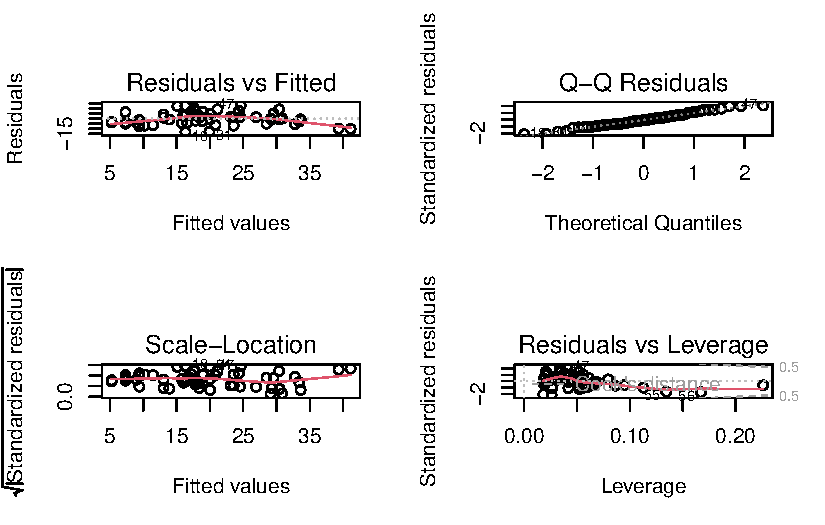
\includegraphics{ENVX2001-2024-Lab07_files/figure-pdf/mlmod-1.pdf}

}

\end{figure}

\begin{Shaded}
\begin{Highlighting}[]
\FunctionTok{par}\NormalTok{(}\AttributeTok{mfrow=}\FunctionTok{c}\NormalTok{(}\DecValTok{1}\NormalTok{,}\DecValTok{1}\NormalTok{))}

\FunctionTok{summary}\NormalTok{(lm.mod1)}
\end{Highlighting}
\end{Shaded}

\begin{verbatim}

Call:
lm(formula = ABUND ~ GRAZE + L10AREA, data = loyn)

Residuals:
     Min       1Q   Median       3Q      Max 
-13.4296  -4.3186  -0.6323   4.1273  13.0739 

Coefficients:
            Estimate Std. Error t value Pr(>|t|)    
(Intercept)  21.6029     3.0917   6.987 4.73e-09 ***
GRAZE        -2.8535     0.7125  -4.005 0.000195 ***
L10AREA       6.8901     1.2900   5.341 1.98e-06 ***
---
Signif. codes:  0 '***' 0.001 '**' 0.01 '*' 0.05 '.' 0.1 ' ' 1

Residual standard error: 6.444 on 53 degrees of freedom
Multiple R-squared:  0.6527,    Adjusted R-squared:  0.6396 
F-statistic: 49.81 on 2 and 53 DF,  p-value: 6.723e-13
\end{verbatim}

This is a significant model as both b1 and b2 are significant and the
model is significant.

The residuals look reasonable. They are approximately normally
distributed (both right hand plots), but possibly the variance is not
totally constant and there are possibly a few values with high leverage
(left hand plots).

\begin{tcolorbox}[enhanced jigsaw, rightrule=.15mm, coltitle=black, leftrule=.75mm, titlerule=0mm, breakable, toprule=.15mm, bottomtitle=1mm, colback=white, toptitle=1mm, opacitybacktitle=0.6, bottomrule=.15mm, arc=.35mm, left=2mm, title=\textcolor{quarto-callout-warning-color}{\faExclamationTriangle}\hspace{0.5em}{Question 3}, colbacktitle=quarto-callout-warning-color!10!white, opacityback=0, colframe=quarto-callout-warning-color-frame]

How good is the model based on the (i) \emph{r}\textsuperscript{2} (ii)
adjusted \emph{r}\textsuperscript{2}? Use \texttt{summary()}.

\end{tcolorbox}

\begin{Shaded}
\begin{Highlighting}[]
\FunctionTok{summary}\NormalTok{(lm.mod1)}\SpecialCharTok{$}\NormalTok{r.squared}
\FunctionTok{summary}\NormalTok{(lm.mod1)}\SpecialCharTok{$}\NormalTok{adj.r.squared  }
\end{Highlighting}
\end{Shaded}

\hypertarget{answer-8}{%
\subsection{Answer}\label{answer-8}}

The Adjusted \emph{r}\textsuperscript{2} is lower than the
\emph{r}\textsuperscript{2}, but we would opt for the adjusted
\emph{r}\textsuperscript{2} as it takes the number of predictors into
account. Overall the model is ok, explaining 64.0\% of variation in
Abundance.

\begin{tcolorbox}[enhanced jigsaw, rightrule=.15mm, coltitle=black, leftrule=.75mm, titlerule=0mm, breakable, toprule=.15mm, bottomtitle=1mm, colback=white, toptitle=1mm, opacitybacktitle=0.6, bottomrule=.15mm, arc=.35mm, left=2mm, title=\textcolor{quarto-callout-warning-color}{\faExclamationTriangle}\hspace{0.5em}{Question 4}, colbacktitle=quarto-callout-warning-color!10!white, opacityback=0, colframe=quarto-callout-warning-color-frame]

Which variable(s) has the most significant effect(s)? \emph{(Refer
specifically to the t probabilities in the table of predictors and their
estimated parameters or coefficients in the output of
\texttt{summary()})}. Interpret the p-values in terms of dropping
predictor variables.

\end{tcolorbox}

\hypertarget{answer-9}{%
\subsection{Answer}\label{answer-9}}

Both \texttt{L10AREA} and \texttt{GRAZE} are highly significant,
\texttt{L10AREA} is the most significant. In terms of effect, a 1 unit
change in \texttt{GRAZE} results in a -2.9 decrease in abundance (with
\texttt{L10AREA} remaining constant), while a 1 unit change in
\texttt{L10AREA}, (therefore a 10 unit change in \texttt{AREA}) results
in a 6.9 increase in abundance (\texttt{GRAZE} holding constant).

\begin{tcolorbox}[enhanced jigsaw, rightrule=.15mm, coltitle=black, leftrule=.75mm, titlerule=0mm, breakable, toprule=.15mm, bottomtitle=1mm, colback=white, toptitle=1mm, opacitybacktitle=0.6, bottomrule=.15mm, arc=.35mm, left=2mm, title=\textcolor{quarto-callout-warning-color}{\faExclamationTriangle}\hspace{0.5em}{Question 5}, colbacktitle=quarto-callout-warning-color!10!white, opacityback=0, colframe=quarto-callout-warning-color-frame]

Repeat the multiple regression, but this time include YRS.ISOL as a
predictor variable (it has the 3rd largest absolute correlation). This
will allow you to assess the effect of YRS.ISOL with the other variables
taken into account.

\end{tcolorbox}

\hypertarget{answer-10}{%
\subsection{Answer}\label{answer-10}}

\begin{Shaded}
\begin{Highlighting}[]
\NormalTok{lm.mod2 }\OtherTok{\textless{}{-}} \FunctionTok{lm}\NormalTok{(ABUND }\SpecialCharTok{\textasciitilde{}}\NormalTok{ GRAZE }\SpecialCharTok{+}\NormalTok{ L10AREA }\SpecialCharTok{+}\NormalTok{ YR.ISOL, }\AttributeTok{data=}\NormalTok{loyn)}
\end{Highlighting}
\end{Shaded}

\begin{tcolorbox}[enhanced jigsaw, rightrule=.15mm, coltitle=black, leftrule=.75mm, titlerule=0mm, breakable, toprule=.15mm, bottomtitle=1mm, colback=white, toptitle=1mm, opacitybacktitle=0.6, bottomrule=.15mm, arc=.35mm, left=2mm, title=\textcolor{quarto-callout-warning-color}{\faExclamationTriangle}\hspace{0.5em}{Question 6}, colbacktitle=quarto-callout-warning-color!10!white, opacityback=0, colframe=quarto-callout-warning-color-frame]

Check assumptions, do the residuals look ok? If you are happy with the
assumptions, you can proceed to interpret the model output.

\end{tcolorbox}

\hypertarget{answer-11}{%
\subsection{Answer}\label{answer-11}}

\begin{Shaded}
\begin{Highlighting}[]
\FunctionTok{par}\NormalTok{(}\AttributeTok{mfrow=}\FunctionTok{c}\NormalTok{(}\DecValTok{2}\NormalTok{,}\DecValTok{2}\NormalTok{))}
\FunctionTok{plot}\NormalTok{(lm.mod2)}
\end{Highlighting}
\end{Shaded}

\begin{figure}[H]

{\centering 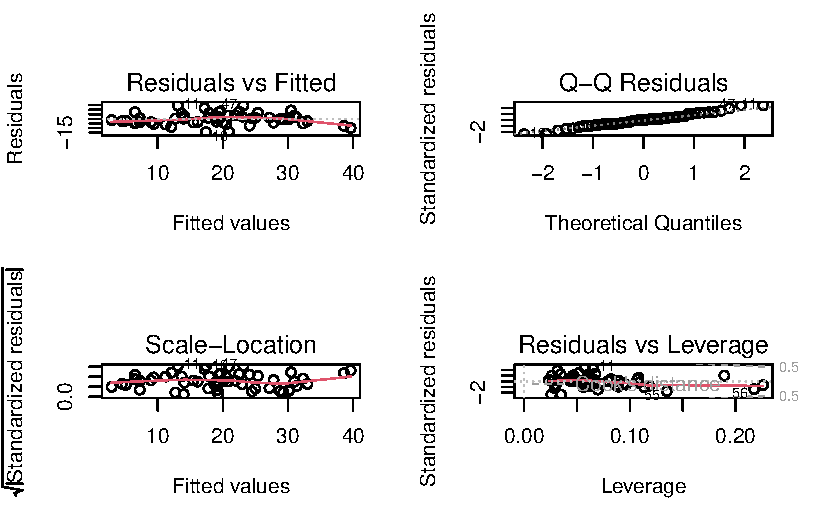
\includegraphics{ENVX2001-2024-Lab07_files/figure-pdf/unnamed-chunk-18-1.pdf}

}

\end{figure}

\begin{Shaded}
\begin{Highlighting}[]
\FunctionTok{par}\NormalTok{(}\AttributeTok{mfrow=}\FunctionTok{c}\NormalTok{(}\DecValTok{1}\NormalTok{,}\DecValTok{1}\NormalTok{))}
\end{Highlighting}
\end{Shaded}

\begin{tcolorbox}[enhanced jigsaw, rightrule=.15mm, coltitle=black, leftrule=.75mm, titlerule=0mm, breakable, toprule=.15mm, bottomtitle=1mm, colback=white, toptitle=1mm, opacitybacktitle=0.6, bottomrule=.15mm, arc=.35mm, left=2mm, title=\textcolor{quarto-callout-warning-color}{\faExclamationTriangle}\hspace{0.5em}{Question 7}, colbacktitle=quarto-callout-warning-color!10!white, opacityback=0, colframe=quarto-callout-warning-color-frame]

Compare the \emph{r}\textsuperscript{2} and adjusted
\emph{r}\textsuperscript{2} values with those you calculated for the 2
predictor model, Which is the better model? Why?

\end{tcolorbox}

\begin{Shaded}
\begin{Highlighting}[]
\FunctionTok{summary}\NormalTok{(lm.mod2)}
\end{Highlighting}
\end{Shaded}

\hypertarget{answer-12}{%
\subsection{Answer}\label{answer-12}}

Both of these are greater than for model in step 3, so this is a better
model.

\hypertarget{at-your-own-time-california-streamflow}{%
\subsection{At your own time: California
streamflow}\label{at-your-own-time-california-streamflow}}

\begin{tcolorbox}[enhanced jigsaw, rightrule=.15mm, coltitle=black, leftrule=.75mm, titlerule=0mm, breakable, toprule=.15mm, bottomtitle=1mm, colback=white, toptitle=1mm, opacitybacktitle=0.6, bottomrule=.15mm, arc=.35mm, left=2mm, title=\textcolor{quarto-callout-note-color}{\faInfo}\hspace{0.5em}{Note}, colbacktitle=quarto-callout-note-color!10!white, opacityback=0, colframe=quarto-callout-note-color-frame]

This additional exercise can be done at your own time. Most of the code
are provided. You will need to run the code and interpret the results.

\end{tcolorbox}

The following dataset contains 43 years of annual precipitation
measurements (in mm) taken at (originally) 6 sites in the Owens Valley
in California. I have reduced this to three variables labelled
\texttt{L10APSAB} (Lake Sabrina), \texttt{L10OBPC} (Big Pine Creek),
\texttt{L10OPRC} (Rock Creek), and the dependent variable stream runoff
volume (measured in ML/year) at a site near Bishop, California (labelled
\texttt{L10BSAAM}). There is also a variable \texttt{Year} but you can
ignore this.

Note the variables have already been log-transformed to increase
normality of the residuals in the regressions.

Start with a full model and manually remove the variables one at a time,
checking every time whether removal of a variable actually improves the
model.

\begin{Shaded}
\begin{Highlighting}[]
\CommentTok{\# read in the data}
\NormalTok{s.data }\OtherTok{\textless{}{-}} \FunctionTok{read\_xlsx}\NormalTok{(}\StringTok{"mlr.xlsx"}\NormalTok{, }\StringTok{"California\_streamflow"}\NormalTok{)}
\FunctionTok{names}\NormalTok{(s.data)}
\end{Highlighting}
\end{Shaded}

\begin{verbatim}
[1] "L10APSAB" "L10OBPC"  "L10OPRC"  "L10BSAAM"
\end{verbatim}

\begin{Shaded}
\begin{Highlighting}[]
\NormalTok{s.mod\_full }\OtherTok{\textless{}{-}}\FunctionTok{lm}\NormalTok{(L10BSAAM}\SpecialCharTok{\textasciitilde{}}\NormalTok{L10APSAB }\SpecialCharTok{+}\NormalTok{ L10OBPC }\SpecialCharTok{+}\NormalTok{ L10OPRC, }\AttributeTok{data=}\NormalTok{s.data)}
\NormalTok{s.mod\_full }\OtherTok{\textless{}{-}}\FunctionTok{lm}\NormalTok{(L10BSAAM}\SpecialCharTok{\textasciitilde{}}\NormalTok{., }\AttributeTok{data=}\NormalTok{s.data) }\DocumentationTok{\#\# you can also use the . to indicate use all variables}
\FunctionTok{summary}\NormalTok{(s.mod\_full)}
\end{Highlighting}
\end{Shaded}

\begin{verbatim}

Call:
lm(formula = L10BSAAM ~ ., data = s.data)

Residuals:
     Min       1Q   Median       3Q      Max 
-0.09885 -0.03331  0.01025  0.03359  0.09495 

Coefficients:
            Estimate Std. Error t value Pr(>|t|)    
(Intercept)  3.25716    0.12360  26.352  < 2e-16 ***
L10APSAB     0.05631    0.03756   1.499  0.14185    
L10OBPC      0.21085    0.06756   3.121  0.00339 ** 
L10OPRC      0.43838    0.08798   4.983 1.32e-05 ***
---
Signif. codes:  0 '***' 0.001 '**' 0.01 '*' 0.05 '.' 0.1 ' ' 1

Residual standard error: 0.04861 on 39 degrees of freedom
Multiple R-squared:  0.8817,    Adjusted R-squared:  0.8726 
F-statistic: 96.88 on 3 and 39 DF,  p-value: < 2.2e-16
\end{verbatim}

\hypertarget{partial-f-tests}{%
\subsubsection{Partial F-Tests}\label{partial-f-tests}}

The above analysis tells us that both \texttt{L10OBPC} \&
\texttt{L10OPRC} are significant, according to the t-test, in the model
and \texttt{L10APSAB} is not? This involves performing Partial F-Tests
as discussed in the lecture.

This can be done in \textbf{R} by using \texttt{anova()} on two model
objects. To be able to compare the models and run the anova, you need to
make objects of all the possible model combinations you want to compare.

\begin{Shaded}
\begin{Highlighting}[]
\NormalTok{s.mod\_reduced }\OtherTok{\textless{}{-}} \FunctionTok{lm}\NormalTok{(L10BSAAM }\SpecialCharTok{\textasciitilde{}}\NormalTok{ L10OPRC }\SpecialCharTok{+}\NormalTok{ L10OBPC, }\AttributeTok{data=}\NormalTok{s.data)}
\FunctionTok{anova}\NormalTok{(s.mod\_reduced, s.mod\_full)}
\end{Highlighting}
\end{Shaded}

The last row gives the results of the partial F-test.

\begin{tcolorbox}[enhanced jigsaw, rightrule=.15mm, coltitle=black, leftrule=.75mm, titlerule=0mm, breakable, toprule=.15mm, bottomtitle=1mm, colback=white, toptitle=1mm, opacitybacktitle=0.6, bottomrule=.15mm, arc=.35mm, left=2mm, title=\textcolor{quarto-callout-warning-color}{\faExclamationTriangle}\hspace{0.5em}{Question 1}, colbacktitle=quarto-callout-warning-color!10!white, opacityback=0, colframe=quarto-callout-warning-color-frame]

Should we remove \texttt{L10APSAB} from the model?

\end{tcolorbox}

\hypertarget{answer-13}{%
\subsection{Answer}\label{answer-13}}

Yes, we should remove L10APSAB as the p-value is \textgreater{} 0.05 and
opt for the simpler model.

\begin{tcolorbox}[enhanced jigsaw, rightrule=.15mm, coltitle=black, leftrule=.75mm, titlerule=0mm, breakable, toprule=.15mm, bottomtitle=1mm, colback=white, toptitle=1mm, opacitybacktitle=0.6, bottomrule=.15mm, arc=.35mm, left=2mm, title=\textcolor{quarto-callout-warning-color}{\faExclamationTriangle}\hspace{0.5em}{Question 2}, colbacktitle=quarto-callout-warning-color!10!white, opacityback=0, colframe=quarto-callout-warning-color-frame]

Is the p-value for the f-test the same as for the t-test?

\end{tcolorbox}

\hypertarget{answer-14}{%
\subsection{Answer}\label{answer-14}}

Yes, P-values for the t-statistic and for the Partial F-statistic are
related (Partial F = t\textsuperscript{2})

\begin{tcolorbox}[enhanced jigsaw, rightrule=.15mm, coltitle=black, leftrule=.75mm, titlerule=0mm, breakable, toprule=.15mm, bottomtitle=1mm, colback=white, toptitle=1mm, opacitybacktitle=0.6, bottomrule=.15mm, arc=.35mm, left=2mm, title=\textcolor{quarto-callout-warning-color}{\faExclamationTriangle}\hspace{0.5em}{Question 3}, colbacktitle=quarto-callout-warning-color!10!white, opacityback=0, colframe=quarto-callout-warning-color-frame]

Write out the hypotheses you are testing.

\end{tcolorbox}

\hypertarget{answer-15}{%
\subsection{Answer}\label{answer-15}}

H\textsubscript{0}: \(\beta_{L10APSAB} = 0\)\\
H\textsubscript{1}: \(\beta_{L10APSAB} \neq 0\)

Perform a Partial F-Test to work out if the removal of \texttt{L10APSAB}
and \texttt{L10OBPC} improves upon the full model.

\begin{Shaded}
\begin{Highlighting}[]
\NormalTok{s.mod\_reduced2  }\OtherTok{\textless{}{-}} \FunctionTok{lm}\NormalTok{(L10BSAAM }\SpecialCharTok{\textasciitilde{}}\NormalTok{ L10APSAB }\SpecialCharTok{+}\NormalTok{ L10OBPC,}\AttributeTok{data=}\NormalTok{s.data)}
\FunctionTok{anova}\NormalTok{(s.mod\_reduced2, s.mod\_full)}
\end{Highlighting}
\end{Shaded}

\begin{verbatim}
Analysis of Variance Table

Model 1: L10BSAAM ~ L10APSAB + L10OBPC
Model 2: L10BSAAM ~ L10APSAB + L10OBPC + L10OPRC
  Res.Df      RSS Df Sum of Sq      F    Pr(>F)    
1     40 0.150845                                  
2     39 0.092166  1   0.05868 24.831 1.321e-05 ***
---
Signif. codes:  0 '***' 0.001 '**' 0.01 '*' 0.05 '.' 0.1 ' ' 1
\end{verbatim}

\begin{tcolorbox}[enhanced jigsaw, rightrule=.15mm, coltitle=black, leftrule=.75mm, titlerule=0mm, breakable, toprule=.15mm, bottomtitle=1mm, colback=white, toptitle=1mm, opacitybacktitle=0.6, bottomrule=.15mm, arc=.35mm, left=2mm, title=\textcolor{quarto-callout-warning-color}{\faExclamationTriangle}\hspace{0.5em}{Question 4}, colbacktitle=quarto-callout-warning-color!10!white, opacityback=0, colframe=quarto-callout-warning-color-frame]

Which variable should be added to the model containing L10OPRC?

\end{tcolorbox}

\hypertarget{answer-16}{%
\subsection{Answer}\label{answer-16}}

L10APSAB does not improve the model with only L10OPRC
(\(\beta_{L10APSAB} = 0\)), so we can say that we should add L10OBPC to
the model containing L10OPRC.

Remember: H0: No difference between the models, so choose the simplest
H1: Full model is better

\begin{tcolorbox}[enhanced jigsaw, rightrule=.15mm, coltitle=black, leftrule=.75mm, titlerule=0mm, breakable, toprule=.15mm, bottomtitle=1mm, colback=white, toptitle=1mm, opacitybacktitle=0.6, bottomrule=.15mm, arc=.35mm, left=2mm, title=\textcolor{quarto-callout-warning-color}{\faExclamationTriangle}\hspace{0.5em}{Question 5}, colbacktitle=quarto-callout-warning-color!10!white, opacityback=0, colframe=quarto-callout-warning-color-frame]

Could things be even simpler? Perform a partial F-Test to see if a model
containing L10OPRC alone could be suitable.

\end{tcolorbox}

\begin{Shaded}
\begin{Highlighting}[]
\NormalTok{s.mod\_reduced3  }\OtherTok{\textless{}{-}} \FunctionTok{lm}\NormalTok{(L10BSAAM }\SpecialCharTok{\textasciitilde{}}\NormalTok{ L10OPRC,}\AttributeTok{data=}\NormalTok{s.data)}
\FunctionTok{anova}\NormalTok{(s.mod\_reduced3, s.mod\_full)}
\end{Highlighting}
\end{Shaded}

\hypertarget{answer-17}{%
\subsection{Answer}\label{answer-17}}

Fitting with only L10OPRC does not improve model fit (P\textless0.05)
and so we can conclude that the better model is the one with L10OBPC and
L10OPRC as predictors, with L10APSAB removed.

\begin{tcolorbox}[enhanced jigsaw, rightrule=.15mm, coltitle=black, leftrule=.75mm, titlerule=0mm, breakable, toprule=.15mm, bottomtitle=1mm, colback=white, toptitle=1mm, opacitybacktitle=0.6, bottomrule=.15mm, arc=.35mm, left=2mm, title=\textcolor{quarto-callout-warning-color}{\faExclamationTriangle}\hspace{0.5em}{Question 6}, colbacktitle=quarto-callout-warning-color!10!white, opacityback=0, colframe=quarto-callout-warning-color-frame]

What is your optimal model?

\end{tcolorbox}

\hypertarget{answer-18}{%
\subsection{Answer}\label{answer-18}}

The best model is:
\(L10BSAAM = \beta_0 + \beta_1 L10OPRC + \beta_2 L10OBPC + error\)

That's it for today! Great work fitting simple and multiple linear
regression! Next week we jump into stepwise selection and predictive
modelling!



\end{document}
